\documentclass{beamer}

% rubber: module pdftex

%\mode<presentation>
%{
%  \usetheme{Boadilla}
%}


\usepackage[finnish]{babel}
\usepackage[utf8]{inputenc}
\usepackage{times}
\usepackage[T1]{fontenc}
\usepackage{amsmath}

\title{Järjestämisalgoritmit}

\subtitle{Superlaskenta kotitietokoneella}

\author{Laura Leppänen}

\date{19. maaliskuuta, 2012}

\begin{document}

\begin{frame}
\titlepage
\end{frame}

\section{Arkkitehtuurin kertausta}

\begin{frame}{Arkkitehtuurin kertausta}{Suorittimet}
  \begin{figure}
    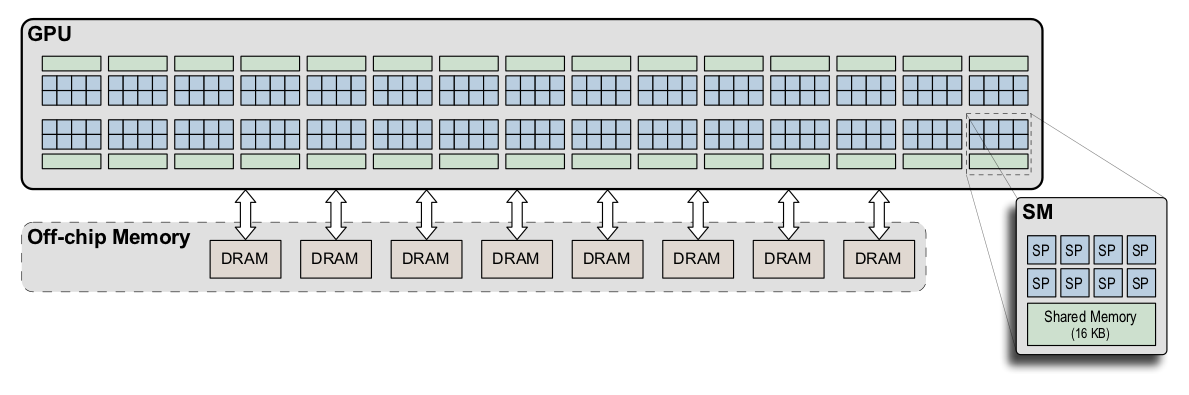
\includegraphics[scale=0.25]{geforce_gtx280.png}
    \caption{Geforce GTX 280}
  \end{figure}

  \begin{itemize}
  \item
    Useita moniprosessoreita (\emph{streaming multiprocessor}), joilla useita ytimiä.
  \item
    Kommunikaatio moniprosessorien välillä hidasta.
    % Tapahtuu tyypillisesti globaalin muistin kautta.
  \end{itemize}
\end{frame}

\begin{frame}{Arkkitehtuurin kertausta}{Säikeiden suoritus}
    \begin{itemize}
    \item
    Säikeet jaetaan lohkoihin ja lohkot 32 säikeen nippuihin (\emph{warp}).
    % Nipun koko riippunee näytönohjainkortista.
    \item
      Samaan nippuun kuuluvat säikeet suorittavat samaa käskyä samaan aikaan.
    \item
      Optimaalisessa tilanteessa kaikki saman nipun säikeet valitsevat saman suorituspolun.
    \item
      Yhtäaikaisia säikeitä tarvitaan paljon (tuhansia).
    \end{itemize}
\end{frame}

\end{document}
